\section{Proof Methods}

\frame{
{Part 2: Proof Methods}

\tableofcontents[currentsection,hideallsubsections, firstsection=2, sections={2-5}]}


\subsection{Concepts}

\begin{frame}
  \frametitle{What is a Proof?}

  \begin{itemize}
  \item \structure{A proposition} is a statement that can be
    \structure{True} or \alert{False}.
    \begin{itemize}
    \item This room has 40 chairs.
    \item Every intelligent being feels pain.
    \item Please say your name.
    \item $513 \times 435 = 223165$
    \item Every even integer greater than 2 is the sum of two primes.
    \item It is raining now.
    \end{itemize}

    \bigskip

  \item A \structure{proof} is a method of proving the truth or falsehood of a proposition.
    \begin{itemize}
    \item \structure{mathematical proofs} normally use logical steps
      to show the truth of a mathematical proposition.
    \end{itemize}
  \end{itemize}

\end{frame}

\begin{frame}
  \frametitle{Proof Examples}
  \begin{itemize}
  \item Pitagoras by pictures
  \item Getting rich with triangles
  \item 1 == -1
  \end{itemize}
\end{frame}

\begin{frame}
  \frametitle{Morals of Proofs}
  \begin{itemize}
  \item Make sure that you are applying the rules properly.
  \item \structure{Mindless calculation} does not replace \structure{understanding}.
  \end{itemize}
\end{frame}


\subsection{Proof Terms}
\begin{frame}
  \frametitle{Common Terms used in Proofs}
  \begin{itemize}
  \item \structure{Proposition}:\\
    \only<2>{A statement that is either true or false}
  \item \structure{Predicate}:\\
    \only<2>{A preposition that depends on variables}
  \item \structure{Axiom}:\\
    \only<2>{A preposition that is accepted to be true}
  \item \structure{Proof}:\\
    \only<2>{A sequence of axioms and proved statements that conclude with the proposition of interest}
  \item \structure{Theorem}:\\
    \only<2>{An important true proposition}
  \item \structure{Lemma}:\\
    \only<2>{A simpler proposition that is useful to prove later propositions}
  \item \structure{Corollary}:\\
    \only<2>{A proposition that follows from a theorem in a few logical steps}
  \end{itemize}
\end{frame}


\begin{frame}
  \frametitle{Our first proof method: Modus Ponens}

  \begin{equation*}
    \frac{P, P \text{ implies } Q}{Q}\text{ or } \frac{P, P\rightarrow Q}{Q}
  \end{equation*}

  \vfill

  \begin{block}{What does ``Modus Ponens'' mean?}

    \begin{itemize}
    \item If P is true.
    \item and if P being true \alert{requires} that Q is true
      too.
    \item then Q is true.
    \end{itemize}
  \end{block}

\end{frame}

\begin{frame}
  \frametitle{How can we use Modus Ponens to prove something?}
  \begin{itemize}
  \item We want to prove Q.
  \item Prove that when P is true, Q \alert{must} be true
  \item Prove that P is true
  \item \structure{therefore}, Q must be true.
  \end{itemize}
\end{frame}

\subsection{Proof by Contradiction}
\begin{frame}
  \frametitle{Proof By Contradiction}

  A trivial proof:

  \begin{equation*}
    \sqrt[3]{1332} \leq 11
  \end{equation*}

\end{frame}

\begin{frame}
  \frametitle{Proof By Contradiction}

  If an assertion \alert{implies something false}

  \bigskip

  Then the \alert{assertion must be false!}
\end{frame}

\begin{frame}
  \frametitle{Better Example: $\sqrt{2}$ is irrational}

  \begin{center}
    Think a little bit by yourselves first.
  \end{center}
\end{frame}

\begin{frame}
  \frametitle{Better Example: $\sqrt{2}$ is irrational}

  Let's prove by contradiction:

  \bigskip

  \begin{enumerate}
  \item Assume that $\sqrt{2}$ is rational
    \bigskip
  \item Therefore $\sqrt{2} = \frac{m}{n}$, and $m$ and $n$ are
    integers with \alert{no common prime factors} ($n\neq0$).
    \bigskip
  \item Therefore $n\sqrt{2} = m$, $2n^2 = m^2$, and $m^2$ is even.
    \bigskip
  \item If $m^2$ is even, then $m$ is even too. $m = 2k$ for some integer $k$.
    \bigskip
  \item Therefore $2n^2 = (2k)^2$, $2n^2 = 4k^2$, $n^2 = 2k^2$, and $n^2$ is even.
    \bigskip
  \item If $n^2$ is even, then $n$ is even too. \alert{$n$ and $m$ are both even (contradiction).}
  \end{enumerate}



\end{frame}

\subsection{Proof by Cases}

\begin{frame}[fragile]
  \frametitle{Proof By Cases}

  Prove that these two code samples are the same:

  \vfill

  \begin{block}{Code 1}
\begin{verbatim}
If (X > 0 OR (X <= 0 AND Y > 100))
  print("Hello!")
\end{verbatim}
  \end{block}
  \begin{block}{Code 2}
\begin{verbatim}
If (X > 0 OR Y > 100)
  print("Hello!")
\end{verbatim}
  \end{block}

\end{frame}

\begin{frame}
  \frametitle{Proof By Cases}

  \begin{itemize}
  \item ``Proof by Cases'' breaks a complicated problem into easier, smaller sub-problems.

    \bigskip

  \item It is important to make sure that \alert{the cases cover all possibilities}, or the
    proof is not complete.
  \end{itemize}
\end{frame}

\begin{frame}
  \frametitle{Proof By Cases: Friends and Strangers}

  \begin{center}
    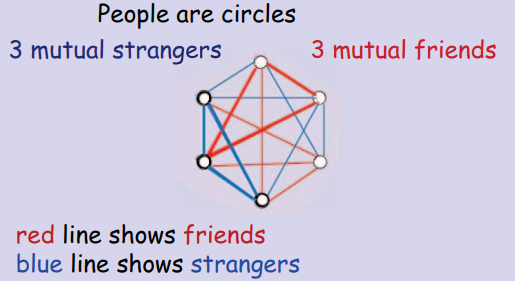
\includegraphics[width=0.8\textwidth]{../img/friends_and_strangers}
  \end{center}

  \begin{itemize}
  \item Six people, every two are either \alert{friends} or \structure{strangers}.
  \item {\bf Claim:} There is always a set of \alert{3 mutual
    friends} or \structure{3 mutual strangers}.
  \end{itemize}

\end{frame}

\begin{frame}
  \frametitle{Friends and Strangers, and Ramsey's Theorem}

  For any $k$, every \structure{large enough group} of people
  will contain $k$ mutual friends OR $k$ mutual strangers.

  \bigskip

  \begin{itemize}
  \item $R(3) = 6$
  \item $R(4) = 18$
  \item $R(5) = \text{ unknown!}$
  \end{itemize}
\end{frame}

\begin{frame}
  \frametitle{A bogus proof by cases: Prove $2a^2 > a$}
  \begin{enumerate}
  \item This proof is by case analysis.
  \item There are two cases:
    \begin{itemize}
      \item Case 1: $a$ is positive
      \item Case 2: $a$ is negative
    \end{itemize}
  \item One of these cases must always hold, because an integer is either positive or negative.
  \item Case 1: Suppose $a$ is positive.
  \item Since $a$ is an integer, we must have that $a \geq 1$.
  \item Hence, $2a^2 = 2a\times a \geq 2a\times 1 > a$.
  \item This implies the claim holds in Case 1.
  \item Case 2: Suppose $a$ is negative.
  \item Since $a$ is an integer, we must have that $a \leq -1$.
  \item Hence, $2a^2 \geq 2\times (-1 \times -1) = 2 > -1 \geq a$.
  \item This implies the claim holds in Case 2.
  \item The claim therefore holds in both cases.
  \end{enumerate}
\end{frame}
